\section[The fundamental projections]{The four fundamental orthogonal projections}
\label{sec:orthproj}

One of the bonuses we reap from the pseudoinverse is the four fundamental orthogonal projections. Each of these matrices projects onto a specific vector space. The spaces are these:
\begin{enumerate}
\item the range $\rng{\A{}}$,
\item the orthogonal complement to the range, $\rng{\A{}}^{\perp}$,
\item the null space $\nll{\A{}}$,
\item the orthogonal complement to the null space, $\nll{\A{}}^{\perp}$.
\end{enumerate}

We can make a simple yet powerful observation about the projectors.
Given the $\pee{}_{\mathcal{V}}$, the projector onto an $m-$dimensional subspace $\mathcal{V}$, the projector onto the orthogonal complement is
\begin{equation}
  \pee{}_{\mathcal{V}^{perp}} = \I{m}-\pee{}_{\mathcal{V}}.
\end{equation}

Below are these projectors for a matrix $\Accmn_{\rho}$ with pseudoinverse $\Ap$:
\begin{equation}
\boxed{
  \begin{array}{lcllcl}
    \projra& = &\rightinv & \quad \projrap& = &\I{m}-\rightinv\\
    \projnap& =& \leftinv & \quad \projna& = &\I{n}-\leftinv\\    
  \end{array}
  }
  \label{eq:fourprojpi}
\end{equation}

%%
\subsection{Projection onto the range of $\A{}$}
Let's explore the matrix product
\begin{equation}
  \begin{split}
    \projra &= \rightinv,\\
    &= \Y{}\,\sig{}\,\sig{(+)}\Y{*},\\
    & = \Y{}\,\J{m}{\rho}\,\Y{*}.
  \end{split}
\end{equation}
The truncated identity is acting like screen which only allows the first $\rho$ column vectors of $\Y{}$ into play. These are the vectors which span the image of the target matrix.

%%
\subsection{Projection onto the orthogonal complement of the range of $\A{}$}
Now subtract this projector from the identity:
\begin{equation}
  \begin{split}
    \projrap& = \I{m}-\projra,\\
      &= \I{m}-\rightinv,\\
      &= \I{m} - \Y{}\,\J{m}{\rho}\,\Y{*}.
  \end{split}
\end{equation}

%%
\subsection{Projection onto the null space of $\A{}$}
\begin{equation}
  \begin{split}
    \projna &= \leftinv,\\
    &= \X{}\,\sig{+}\,\sig{}\X{*},\\
    & = \X{}\,\J{n}{\rho}\,\X{*}.
  \end{split}
\end{equation}The truncated identity is acting like screen which only allows 
%%
\subsection{Projection onto the orthogonal complement of the null space of $\A{}$}
Let's explore the matrix product
\begin{equation}
  \begin{split}
    \projnap& = \I{n}-\projna,\\
      &= \I{n}-\leftinv,\\
      &= \I{n} - \X{}\,\J{n}{\rho}\,\X{*}.
  \end{split}
\end{equation}

Below are the same projectors shown in \eqref{eq:fourprojpi} for the same matrix $\Accmn_{\rho}$ with \svdl\ $\svd{*}$:
\begin{equation}
\boxed{
  \begin{array}{lcllcl}
    \projra&  = &\pra{*}  & \qquad  \projrap & = & \I{m}-\pra{*}\\[3pt]
    \projnap& = &\pnap{*} & \qquad  \projna  & = & \I{n}-\pnap{*}\\    
  \end{array}
  }
  \label{eq:fourprojsvd}
\end{equation}

%%%
%%%
\subsection{Primitive example}
Consider the following simple matrix:
\begin{equation}
  \A{}= \mat{cc}{1&0\\0&1\\0&0}.
\end{equation}
Using SVD by inspection we write
\begin{equation}
\begin{split}
  \svda{T},\\
  &= \I{3}\, \A{}\, \I{2},\\
  &= \mat{cc>{\columncolor{ltgray}}c}{1&0&0\\0&1&0\\0&0&1} \mat{cc}{1&0\\0&1\\\hline0&0} \itwo.
\end{split}
\end{equation}
The pseudoinverse is then
\begin{equation}
  \begin{split}
     \mpgia{T}, \\
     & = \itwo \mat{cc|c}{1&0&0\\0&1&0} \mat{ccc}{1&0&0\\0&1&0\\\rowcolor{ltgray}0&0&1},\\
     & = \mat{ccc}{1&0&0\\0&1&0}.
  \end{split}
\end{equation}

The fundamental spaces are revealed in the SVD and listed in table \eqref{tab:proj:ff}.
\begin{table}[htdp]
\begin{center}
\begin{tabular}{lll}
 subspace & \qquad \qquad span & source\\\hline
 $\rng{\A{}}$  & $\spn\lst{\mat{c}{1\\0\\0},\mat{c}{0\\1\\0}}$ \qquad & $\spn\lst{\Y{}_{*,1},\Y{}_{*,2}}$\\[19pt]\hline
 $\nll{\A{T}}$ & $\spn\lst{\mat{c}{0\\0\\1}}$ & $\spn\lst{\Y{}_{*,3}}$ \\[19pt]\hline
 $\rng{\A{T}}\qquad $ & $\spn\lst{\mat{c}{1\\0},\mat{c}{0\\1}}$ & $\spn\lst{\X{}_{*,1},\X{}_{*,2}}$\\[13pt]\hline
 $\nll{\A{}}$  & \qquad \qquad  $\emptyset$ & \quad  \quad $\emptyset$\\[2pt]\hline
\end{tabular}
\end{center}
\label{tab:proj:ff}
\caption{The fundamental spaces are revealed in the SVD. The codomain matrix $\Y{}$ encodes the vector spaces for the range of $\A{}$, $\rng{\A{}}$ and  the null space of the transpose, $\nll{\A{T}}$. The domain matrix $\X{}$ encodes the vector spaces for the range of the transpose $\A{T}$, $\rng{\A{T}}$ and  the null space of $\A{}$, $\nll{\A{}}$.}
\end{table}%

The analagous projectors are shown in table \eqref{tab:proj:fp}. The projection operators are these:
\begin{equation}
  \begin{array}{lcllcl}
    \projra& = &\rightinv = \mat{ccc}{1&0&0\\0&1&0\\0&0&0} & \quad \projrap& = &\I{m}-\projra = \mat{ccc}{0&0&0\\0&0&0\\0&0&1}\\
    \projnap& =& \leftinv = \itwo & \quad \projna& = &\I{n}-\projnap = \mat{cc}{0&0\\0&0}\\    
  \end{array}
  \label{eq:primitives}
\end{equation}
%%
\begin{table}[htdp]
\begin{center}
\begin{tabular}{llc}
 projection \\
 onto & \qquad vector space & projector\\\hline
 $\rng{\A{}}$  & $\spn\lst{\mat{c}{1\\0\\0},\mat{c}{0\\1\\0}}$ \qquad & $\mat{ccc}{1&0&0\\0&1&0\\0&0&0}$\\[19pt]\hline
 $\rng{\A{}}^{\perp}$ & $\spn\lst{\mat{c}{0\\0\\1}}$ & $\mat{ccc}{0&0&0\\0&0&0\\0&0&1}$ \\[19pt]\hline
 $\nll{\A{T}}\qquad $ & $\spn\lst{\mat{c}{1\\0},\mat{c}{0\\1}}$ & $\itwo$\\[13pt]\hline
 $\nll{\A{T}}^{\perp}$  & \qquad \qquad  $\emptyset$ & $\emptyset$\\[2pt]\hline
\end{tabular}
\end{center}
\label{tab:proj:fp}
\caption{The four fundamental projectors constructed from the target matrix $\A{}$ and the pseudoinverse $\A{T}$.}
\end{table}%

Study the action of the projectors on arbitrary vectors from the domain and the codomain. Because the target matrix is row rank deficient, there will be a null space as shown by the shaded column in the $\Y{}$ matrix. For the codomain the projection actions are these:
\begin{equation}
  \projra (y) = \mat{ccc}{1&0&0\\0&1&0\\0&0&0} 
     \mat{c}{y_{1}\\y_{2}\\y_{3}} = \mat{c}{y_{1}\\y_{2}\\0},
     \label{eq:mpp:red}
\end{equation}
\begin{equation}
  \projrap (y) = \mat{ccc}{0&0&0\\0&0&0\\0&0&1} 
     \mat{c}{y_{1}\\y_{2}\\y_{3}} = \mat{c}{0\\0\\y_{3}}.
     \label{eq:mpp:blue}
\end{equation}
The first case shows that the operator $\projra$ acts on vectors and projects them onto the $y_{1}-y_{2}$ plane. The complementary operator $\projra$ projects onto $y_{3}$ axis. These actions are shown graphically in figure \eqref{fig:projections3d}.

The case for the domain projection is trivial because the target matrix has full column rank.
\begin{equation}
  \projnap (x) = \itwo \mat{c}{x_{1}\\x_{2}} = \mat{c}{x_{1}\\x_{2}}.
\end{equation}

\begin{figure}[htbp] %  figure placement: here, top, bottom, or page
   \centering
   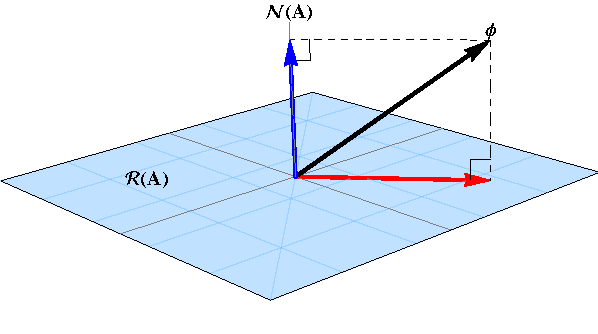
\includegraphics[]{pdf/mpp/projections} 
   \caption{Codomain projection examples. An arbitrary vector $\phi$ is represented by the black arrow. The red arrow shows the orthogonal projection onto the range of $\A{}$ as given by $\projra\paren{\phi}$ as shown in equation \eqref{eq:mpp:red}. The blue arrow shows the orthogonal projection onto the perpendicular complement of range of $\A{}$ as given by $\projrap\paren{\phi}$ as shown in equation \eqref{eq:mpp:blue}.}
   \label{fig:projections3d}
\end{figure}

%%
\subsection{Canonical example}
To solidify the theory work through one more example explicitly. This will show both formulations of the four fundamental projectors: using the pseudoinverse and using the component matrices from \svdl.

Start with the target matrix and the pseudoinverse:s 
\begin{equation}
  \A{} = \Aexample, \quad \Ap = \Aexamplepi.
\end{equation}

The projection onto the range of $\A{}$ is calculated in two different ways.
\begin{equation}
\begin{split}
  \projra &= \leftinv = \rthree
    \mat{rrr}
    { 
    1 & -1 &  1\\
   -1 &  1 & -1\\
    1 & -1 &  1\\
    }.
\end{split}
\end{equation}
However, we can bypass assembling the pseudoinverse and work directly with the decomposition matrices like so:
\begin{equation}
\begin{split}
  \projra &= \Y{}\,\sig{}\,\sig{(+)}\Y{T},\\
    & = \Y{}\,\J{m}{\rho}\,\Y{T},\\
    &= \Yshade \mat{ccc}{1&0&0\\0&0&0\\0&0&0} \Ytshade,\\
    &= \rthree
    \mat{rrr}
    { 
    1 & -1 &  1\\
   -1 &  1 & -1\\
    1 & -1 &  1\\
    }.
\end{split}
\end{equation}

The projection onto the perpendicular complement space  is this
\begin{equation}
  \projrap = \I{3} - \projra = \rthree
    \mat{rrr}
    { 2 & -1 &  1\\
     -1 &  2 & -1\\
      1 & -1 &  2}.
\end{equation}

Let's look at the action of these projectors.
\begin{equation}
  \projra(y) = \rthree
    \mat{rrr}
    { 1 & -1 &  1\\
     -1 &  1 & -1\\
      1 & -1 &  1}
    \mat{c}{y_{1}\\y_{2}\\y_{3}}
    = \rthree \mat{r}{y_{1}-y_{2}+y_{3}\\-y_{1}+y_{2}-y_{3}\\y_{1}-y_{2}+y_{3}}
\end{equation}
If we define
\begin{equation}
  \zeta = \rthree \paren{y_{1}-y_{2}+y_{3}}
\end{equation}
we can write
\begin{equation}
  \projra(y) = \zeta\mat{r}{1\\-1\\1}.
\end{equation}
The is, we are projecting onto a line. The same line so in equation \eqref{} in fact.

\begin{equation}
  \projrap(y) = \rthree
    \mat{rrr}
    { 2 & -1 &  1\\
     -1 &  2 & -1\\
      1 & -1 &  2}
    \mat{c}{y_{1}\\y_{2}\\y_{3}}
    = \rthree \mat{c}{2y_{1}-y_{2}+y_{3}\\-y_{1}+2y_{2}-y_{3}\\y_{1}-y_{2}+2y_{3}}
\end{equation}


\section{A survey of the four fundamental projectors}
In the following pages we will look at three different kinds of mappings for a matrix $\Acc{m}{n}$: no frustration, frustration in one direction, frustration in both directions.

There are two different ways to view frustrated\index{frustration} mappings:
\begin{enumerate}
\item geometric deficiency\index{geometric deficiency} - mapping into a lower dimensional object;
\item algebraic deficiency\index{algebraic deficiency} - rank deficiency in row or column.
\end{enumerate}

In the examples that follow we will see ellipses mapped into other ellipses. These mappings are not frustrated. But once we map into a lower dimensional object, say from the unit sphere onto a line, the map is frustrated. This also means that we can't reverse the map. We can't make a finite linear map from a line with one parameter onto a sphere with three parameters.

These tables specify critical properties of the target matrix.

\textbf{Plots: }All plots start with the unit circle which is either
\begin{equation}
  \begin{array}{rcll}
     S(\theta) &=& \mat{c}{\cos \theta\\\sin \theta},\ \theta\in[0,2\pi) \qquad &n=2,\\
     S(\theta,\phi) &=& \mat{c}{\cos \theta\sin \phi\\\sin \theta \sin \phi\\\cos \phi},\ \theta\in[0,2\pi),\ \phi\in[0,\pi), \qquad &n=3.
  \end{array}
\end{equation}
Then look at the mapping action of the matrix. The result is either
\begin{equation}
  \A{}S(\theta) 
\end{equation}
when the target matrix has two columns or
\begin{equation}
  \A{}S(\theta,\phi) 
\end{equation}
when the target matrix has three columns.

The circles and ellipses have the color determined the the angular variable to provide an clearer idea of how the unit circle is distorted. So for the color red starts at $\theta=0$ and progresses through the spectrum until $\theta=2pi$ where the color is violet.\\

\textbf{Matrix images:} This block summarizes the plot above. For example, it may say that the plot represents a unit sphere being mapped to a line.\\

%%
\textbf{Vector space mappings:} These mappings are based on the dimensions of the spaces for the row and column vectors, $m$ and $n$. They disregard the issue of rank and and concerned purely with the mappings $\real{m}\mapsto\real{n}$ and  $\real{n}\mapsto\real{m}$. This map addresses the geometric deficiency of the mappings. For example are we going from a plane to a plane or a plane to a line. If the map is into a higher dimensional space we will have a frustrated map.\\

\textbf{Matrix ranks:} Are there rank deficiencies in the row or column space? If there is a rank deficiency we will see a frustrated map. 


\clearpage

%%
%% 2 x 2
%%
\begin{table}[htdp]
\begin{center}
\begin{tabular}{cc}
  $\A{}x=y$ & $\A{T}y=x$\\
$\mat{rr}{1&2\\-1&2}\mat{c}{x_{1}\\x_{2}} = \mat{c}{y_{1}\\y_{2}}$ &
$\mat{rr}{1&-1\\2&2}\mat{c}{x_{1}\\x_{2}} = \mat{c}{y_{1}\\y_{2}}$ \\
\ \\
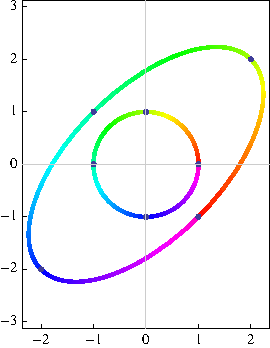
\includegraphics[ width = 2.15in ]{pdf/post_mortemII/2_2_2} &
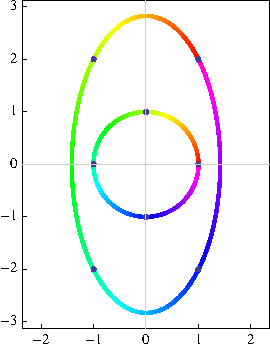
\includegraphics[ width = 2.15in ]{pdf/post_mortemII/2_2_2_t} \\
%%
\ \\
 $\Ap = \frac{1}{4}\mat{rr}{2&-1\\2&1}$ & $\paren{\A{T}}^{+} = \frac{1}{4}\mat{rr}{2&2\\-1&1}$ \\
\ \\
 $\projra = \itwo$ & $\projrat = \itwo$ \\
\ \\
 $\projrap = \mat{cc}{0&0\\0&0}$ & $\projratp = \mat{cc}{0&0\\0&0}$ \\
\ \\
 $\projna = \itwo$ & $\projnat = \itwo$ \\
\ \\
 $\projnap = \mat{cc}{0&0\\0&0}$ & $\projnatp = \mat{cc}{0&0\\0&0}$ \\
\end{tabular}
\end{center}
\label{tab:proj:a}
\caption{The four fundamental projectors for a full rank matrix and its transpose. There is no null space for either $\A{}$ or $\A{T}$.}
\end{table}%

\clearpage
%%
%% 2 x 3
%%
\begin{table}[htdp]
\begin{center}
\begin{tabular}{cc}
  $\A{}x=y$ & $\A{T}y=x$\\
$\mat{ccc}{0&3&0\\1&1&2}\mat{c}{x_{1}\\x_{2}\\x_{3}} = \mat{c}{y_{1}\\y_{2}}$ &
$\mat{cc}{0&1\\3&1\\0&2}\mat{c}{y_{1}\\y_{2}} = \mat{c}{x_{1}\\x_{2}\\x_{3}}$ \\
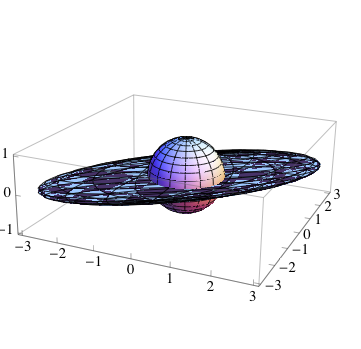
\includegraphics[ width = 2.5in ]{pdf/post_mortemII/3_2_2.png} &
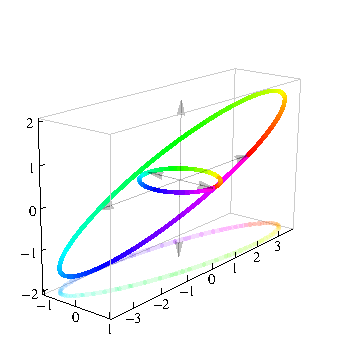
\includegraphics[ width = 2.5in ]{pdf/post_mortemII/3_2_2_t} \\
%%
 $\Ap = \frac{1}{15}\mat{rr}{-2&3\\5&0\\-4&2}$ & $\paren{\A{T}}^{+} = \frac{1}{5}\mat{rrr}{-2&5&-4\\3&0&2}$ \\
\ \\
 $\projra = \itwo$ & $\projrat = \frac{1}{5}\mat{ccc}{1&0&2\\0&1&0\\2&0&4}$ \\
\ \\
 $\projrap = \mat{cc}{0&0\\0&0}$ & $\projratp = \frac{1}{5}\mat{rrr}{4&0&-2\\0&\phantom{-}0&0\\-2&0&1}$ \\
\ \\
 $\projna = \frac{1}{5}\mat{ccc}{1&0&2\\0&1&0\\2&0&4}$ & $\projnat = \itwo$ \\
\ \\
 $\projnap = \frac{1}{5}\mat{rrr}{4&0&-2\\0&\phantom{-}0&0\\-2&0&1}$ & $\projnatp = \mat{cc}{0&0\\0&0}$ \\[15pt]
\end{tabular}
\end{center}
\label{tab:proj:b}
\caption{The four fundamental projectors for a matrix with full row rank. Because the target matrix has full row rank the range spans the domain space and  there is no perpendicular complement.}
\end{table}

\clearpage
%%
%% 3 x 2
%%
\begin{table}[htdp]
\begin{center}
\begin{tabular}{cc}
  $\A{}x=y$ & $\A{T}y=x$\\
$\Aexample \mat{c}{x_{1}\\x_{2}} = \mat{c}{y_{1}\\y_{2}\\y_{3}}$ &
$\Atexample\mat{c}{x_{1}\\x_{2}\\x_{3}} = \mat{c}{y_{1}\\y_{2}}$ \\
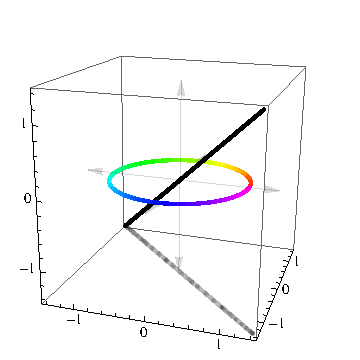
\includegraphics[ width = 2.5in ]{pdf/post_mortemII/3_2_1_a} &
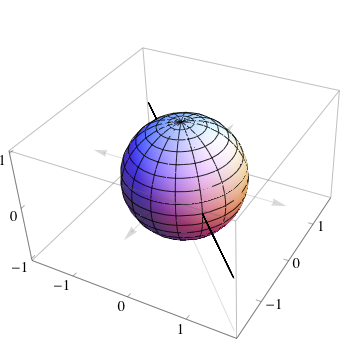
\includegraphics[ width = 2.5in ]{pdf/post_mortemII/3_2_1_t_a} \\
%%
 $\Ap = \Aplus$ & $\paren{\A{T}}^{+} = \frac{1}{6}\Aexample$ \\
\ \\
 $\projra = \frac{1}{3}\Aexample$ & $\projrat = \frac{1}{2}\mat{rr}{1&-1\\-1&1}$ \\
\ \\
 $\projrap = \frac{1}{3}\mat{rrr}{2&1&-1\\1&\phantom{-}2&1\\-1&1&2}$ & $\projratp = \frac{1}{2}\mat{rr}{1&1\\1&1}$ \\
\ \\
 $\projna = \frac{1}{2}\mat{rr}{1&-1\\-1&1}$ & $\projnat = \frac{1}{3}\Aexample$ \\
\ \\
 $\projnap = \frac{1}{2}\mat{rr}{1&1\\1&1}$ & $\projnatp = \frac{1}{3}\mat{rrr}{2&1&-1\\1&\phantom{-}2&1\\-1&1&2}$ \\[10pt]
\end{tabular}
\end{center}
\label{tab:proj:c}
\caption{The four fundamental projectors for a matrix with both row and column rank deficiences. Because the target matrix has full row rank the range spans the domain space and  there is no perpendicular complement.}
\end{table}
\clearpage
\endinput


	
\endinput